\documentclass[pdftex,11pt,a4paper]{book}

\usepackage[spanish]{babel}
\usepackage[utf8]{inputenc}
\usepackage[pdftex]{graphicx}
\usepackage{url}
\usepackage[top=1.5in, bottom=1in, left=1in, right=1in]{geometry}
\usepackage{hyperref}
\usepackage{cite}
\usepackage{float}
\usepackage{eurosym} % para el euro
\usepackage{enumerate}
\usepackage{listings}    
\usepackage{verbatim}


\newcommand{\HRule}{\rule{\linewidth}{0.5mm}}

\renewcommand\figurename{Imagen}


\begin{document}

\begin{titlepage}
\begin{center}

% Upper part of the page. The '~' is needed because \\
% only works if a paragraph has started.
% -----
%
\includegraphics[width=0.35\textwidth]{img/marca-uji-2955.png}~\\[2cm]

\includegraphics{img/marca-uji-2955.png}~\\[3.0cm]

\textsc{\LARGE Grado en Ingeniería Informática}\\[1.5cm]

\textsc{\LARGE Diseño e Implementación de Sistemas de Información}\\[1.5cm]
%%%%%%\textsc{\LARGE Versión Provisional}\\[1.5cm]

% Title
\HRule \\[0.4cm]
{ \huge \bfseries Sistema de soporte a la gestión de la Asignación de Proyectos en Empresas \\[0.4cm] }

\HRule \\[1.5cm]

% Author and supervisor
\begin{minipage}{0.4\textwidth}
\begin{flushleft} \large
\emph{Autor:}\\
Víctor \textsc{Sánchez Terrasa}
\end{flushleft}
\end{minipage}
\begin{minipage}{0.4\textwidth}
\begin{flushright} \large
\emph{Tutor académico:} \\
María de los Ángeles \textsc{López Malo}
\end{flushright}
\end{minipage}

\vfill

% Bottom of the page
% -----
% Sustituir los signos "\_" por lo que corresponda. 
{\large Fecha de lectura: 14 de noviembre de 2018\\
Curso académico 2018/2019}

\end{center}
\end{titlepage}
\setlength{\parskip}{\baselineskip}



% ------------------- Página resumen ---------------------

\thispagestyle{empty} % página sin numerar

\clearpage % Resumen y Palabras clave en página 2.

\section*{Resumen}

En el grado de Ingeniería Informática se necesita un sistema que pueda dar soporte a la gestión de las estancias en prácticas, en estas estancias se incluye también el TFG y la defensa el mismo ante el tribunal, aunque en este caso el alcance del proyecto sólo llegará a la gestionar la asignación de los estudiantes a una estancia en prácticas. 

En este documento se encuentra la descripción del proceso de la elaboración del proyecto incluyendo la definición de requisitos, el análisis del diseño de la aplicación, análisis del diseño de la interfaz y la planificación llevada a cabo.

\thispagestyle{empty} % página sin numerar

\cleardoublepage


% ------------------- Página índice ---------------------


\pagestyle{plain} % todas las páginas numeradas, sin cabeceras. Sustituir por \pagestyle{headings} para añadir cabeceras a las páginas. 

\tableofcontents

\cleardoublepage

% ------------------- Cuerpo de la memoria ---------------------

\chapter{Introducción}

\section{Contexto del proyecto}

En el grado de Ingeniería Informática se necesita un sistema que pueda dar soporte a la gestión de las estancias en prácticas, en estas estancias se incluye también el TFG y la defensa el mismo ante el tribunal, aunque en este caso el alcance del proyecto sólo llegará a la gestionar la asignación de los estudiantes a una estancia en prácticas.

\section{Motivación del proyecto}

El objetivo principal, y estratégico, de este producto es proporcionar apoyo a la gestión propia de la asignatura EI1054: Estancias y Trabajo Final de Grado (TFG) de Ingeniería en Informática \cite{caspractic}.

A nivel táctico y operativo el producto permite agilizar y mejorar la gestión propia de la asignatura EI1054 (Estancias en prácticas y trabajo final de grado). Proporciona un entorno accesible a las empresas y los supervisores para que la gestión de los TFG se pueda llevar a cabo de manera más colaborativa. Facilita el trabajo de revisión y de aceptación de propuestas de TFG. Mejora la publicación y consulta de las ofertas para la realización de los TFG del grado. Finalmente, proporciona transparencia en el proceso de las asignaciones de estancias y TFG.

SAPE se usa únicamente para gestionar las estancias y el TFG del grado de Ingeniería Informática una vez las empresas han creado una oferta para el grado en el sistema central de gestión de la UJI: el IGLU. SAPE se conecta con IGLU para evitar duplicidades de tareas y facilitar el trabajo de la CEiTFG y los CCG. 

En SAPE el usuario principal, y propietarios del producto, es la CEiTFG. Además, son usuarios directos a los alumnos matriculados en la asignatura EI1054, los CCG y las personas de contacto de las empresas. Finalmente, los profesores tutores y los supervisores de las estancias en las empresas son usuarios que sólo reciben información.

SAPE incluye la siguiente funcionalidad:
\begin{itemize}
\item Cuando una empresa introduzca una oferta de estancias para EI en IGLU, deberá acceder a SAPE y completar los datos del TFG. La conexión será automática con el mismo usuario y pwd que tienen dado de alta en el IGLU.
\item La CEiTFG y los CCG puede aprobar propuestas y solicitar cambios o mejoras. SAPE generar una orden para el envío de mails a los contactos de las empresas. Los mails indica qué información se ha pedido y se registrará los datos del envío para que quede constancia.
\item La CEiTFG y los CCG podrán modificar y rechazar propuestas, registrando el motivo. SAPE generará una orden para el envío de un mail que informe la persona de contacto de la empresa del hecho y del motivo, y registrará información del envío para qué quede constancia.
\item Las personas de contacto de las empresas podrán modificar sus propuestas, mientras no estén aceptadas, usando el mismo usuario y pwd que tienen dado de alta en IGLU.
\item En una fecha establecida, la CEiTFG podrá hacer públicas las propuestas revisadas y aprobadas que hage en SAPE hasta esa fecha. Se podrán añadir propuestas aprobadas con posterioridad.
\item Los alumnos matriculados en la asignatura podrán consultar las propuestas de proyectos y la información de interés sobre las empresas.
\item Los alumnos podrán indicar sus preferencias de manera ordenada incluyendo comentarios.
\item La CEiTFG podrá asignar una propuesta de proyecto y un tutor a un alumno. Para poder hacer esta asignación podrán consultar cuál es la ordenación de los alumnos segundo su expediente académico en IGLU.
\item Los alumnos podrán consultar la propuesta de asignación provisional y tendrán un plazo para pedir cambios. Estas solicitudes de cambio quedarán registradas junto con la propuesta inicial.
\item La CEiTFG podrá revisar los cambios solicitados, hacer cambios y volver a publicar la propuesta.
\item La CEiTFG podrá anular una propuesta de asignación para solucionar incidencias puntuales.
\item La CEiTFG podrá activar el traspaso al IGLU de las asignaciones aceptadas.

\end{itemize}

Todas estas funcionalidades no se encuentran el la aplicación, dado que alguna de ellas son complementarias y opcionales dependiendo del número de miembros del grupo escogiendo cuales implementar.

%\section{Estructura de la memoria}

%En este documento se encuentran las etapas del desarrollo de la aplicación pudiendo encontrar en el capítulo 2 la definición del proyecto, como también los requisitos y una descripción de las principales tecnologías usadas en el proyecto, junto con su motivo de uso. El capítulo 3 muestra la metodología que la empresa emplea, la misma empleada en el proyecto, así como también la planificación y el seguimiento que se ha realizado del proyecto. En el capítulo 4 ya se encuentra más información de campo de la informática como el análisis realizado por la aplicación, además del diseño realizado posteriormente del análisis, tanto de la arquitectura del sistema, como de la interfaz. El documento continúa con el capítulo 5 en el que se muestra la implementación de la aplicación, como la puesta en marcha y los errores encontrados en ésta. Finalmente, en el capítulo 6, se tiene a disposición las conclusiones del producto.

\chapter{Diseño de la base de datos}

\section{Modelo UML proporcionado en clase}

Para un correcto desarrollo de la base de datos del proyecto es necesario un modelo UML donde apoyarse. Se parte del modelo del enunciado que se muestra en la Figura \ref{uml_enunciado}.

\begin{figure}[h]
\begin{center}
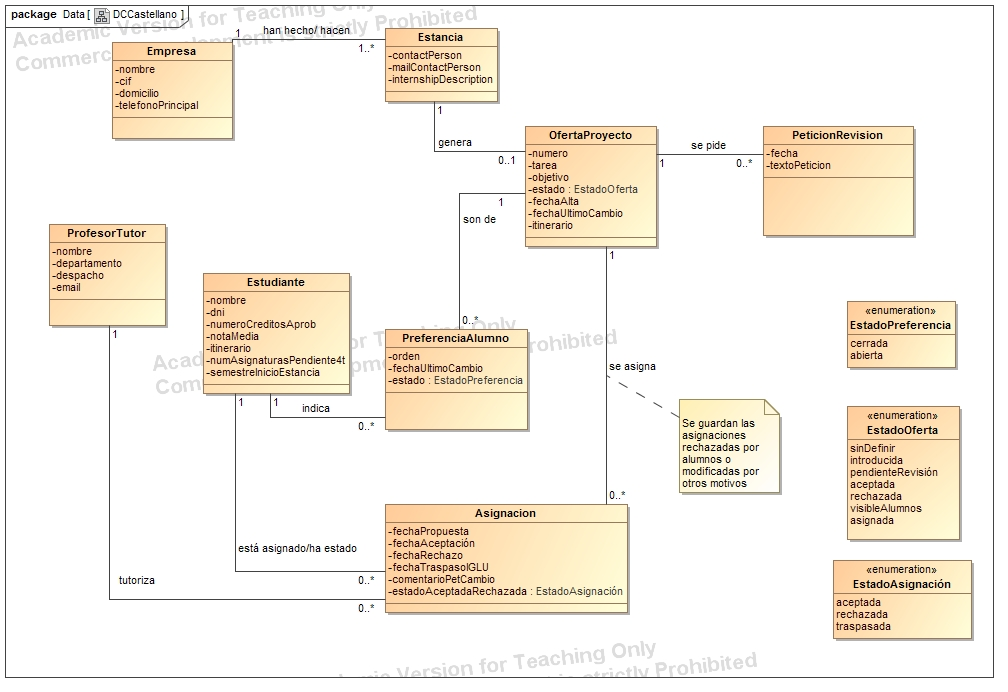
\includegraphics[width=\textwidth]{img/uml_enunciado.jpg}
\caption{\label{uml_enunciado} UML propuesto en el enunciado\cite{caspractic}.}
\end{center}
\end{figure}

\begin{figure}[]
\begin{center}
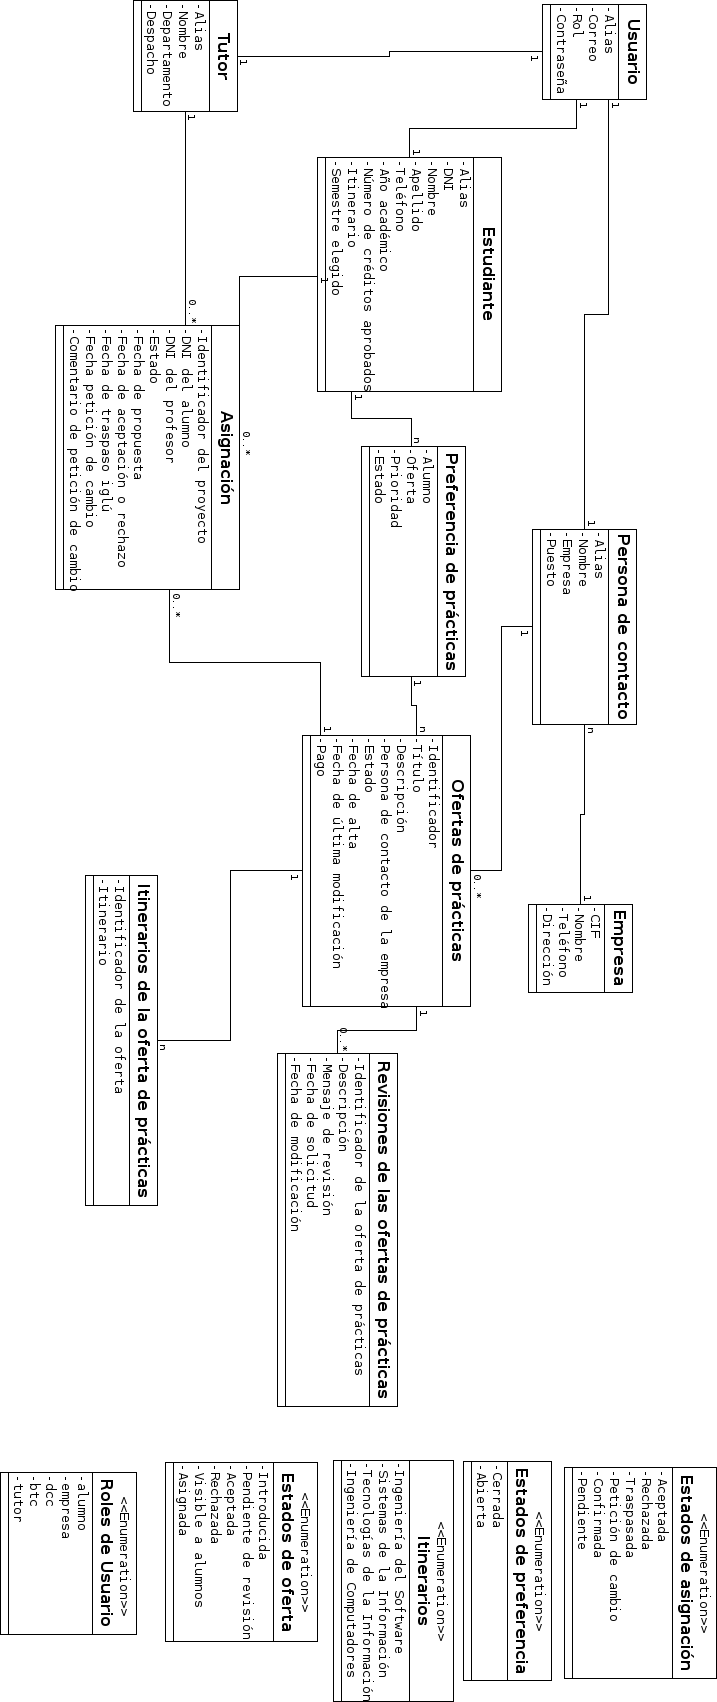
\includegraphics[width=\textwidth]{img/uml_propio}
\caption{\label{uml_propio} UML creado a partir del expuesto en el enunciado.}
\end{center}
\end{figure}

\section{Modelo UML definido para nuestro proyecto}

Con el modelo ofrecido en el apartado anterior, se ha decidido generar el nuestro propio modelo UML de nuestro proyecto. Como se puede visualizar en la Figura \ref{uml_propio} nuestro modelo UML tiene cierta semejanza al modelo del enunciado que se muestra en la Figura \ref{uml_enunciado}.

El mismo modelo UML se también representa el diseño lógico de la base de datos que se emplea en el proyecto donde se encuentran las relaciones entre las tablas, así como los datos primarios y básicos necesitados para el funcionamiento.

\section{Diseño físico}

Partiendo del modelo UML definido, se han escrito los comandos de la base de datos necesarios para el desarrollo del diseño físico que corresponde. en Este diseño es necesario que se incluyen todas las clases descritas anteriormente en el diseño lógico además de las relaciones y reglas de borrado y actualización

\lstinputlisting[language=SQL]{disenyo_trabajo.sql}

\chapter{Diseño de interfaces de usuario.}

Para el diseño de interfaces de usuario se ha hecho un proceso de diseño centrado en el usuario en el que hemos llevado a cabo los siguientes pasos:
\begin{itemize}
\item \textbf{Planificación:} En este punto se identifican los objetivos del sitio web, las necesidades, requerimientos y objetivos de los usuarios, aparte de los objetivos técnicos, equipo de trabajo y presupuesto.

\item \textbf{Diseño conceptual:} Se hizo el sistemas del proyecto desarrollado en el que se ven las diferentes opciones a la hora de navegar por la página web desarrollada según el tipo de rol, que tengas dentro del proyecto ya sea empresa, DCC, BTC o un alumno.

\item \textbf{Diseño visual y definición de estilos:} se acordó una serie de características visuales que se mantienen durante todas las páginas por las que se pueden navegar a amas de otras características individuales, así como también se ven los distintos test realizados, tantos de usuario como heurísticos.

\end{itemize}

\section{Planificación}
La planificación se ha inició primero realizando una lectura en grupo para analizar correctamente cuales son los requisitos que requiere el usuario. Para esto se decidió realizar una reunión todos juntos para poder de definir correctamente los objetivos del proyecto y las áreas de actuación de cada uno.

En esta misma reunión se separaron las áreas de actuación para poder repartir equitativamente las horas que requiere el proyecto.
La área de actuación de Joshua se traté de la parte de realización del funcionamiento lógico de la aplicación en sincronización con Víctor, mientras Joaquín y Paula se encargan de toda la parte visual. Entre todos se realiza tanto la memoria como la documentación técnica que se ha de entregar posterior mente y Paula se encarga de coordinar el grupo comprobando que las tareas se van realizando semanalmente.

Además de todo esto quedamos en reunirnos todos los miércoles para poner en conjunto el trabajo realizado. Estas reuniones ha permitido realizar un gráfico en el que se muestra el avance del trabajo lo largo de las semanas. También se crea un grupo de whatsapp para la comunicación y una carpeta de drive para poner en común el trabajo realizado.

Este proyecto al emplearse como recuperación, Víctor se encarga de solucionar los fallos que se encuentran en la actual memoria, de los fallos de diseño y aplicación. Así también se realiza una tutoría con la profesora para comprobar el avance de la memoria y solucionar tanto dudas como fallos cometidos.

\section{Diseño conceptual}

Respecto al diseño conceptual, se pensó en una aplicación que según el rol detectado por el sistema al introducir el usuario, aparezca una página la cual es requerida por el usuario.

A partir de este punto, dependiendo del rol que tiene el usuario, se vuelven a separar las páginas a las que puede acceder el usuario, variando en según el punto en el que se encuentra el usuario.

De una forma más gráfica que encontramos en la Figura \ref{mapa_web} el mapa web el cual se ha diseñado para toda la plataforma, donde se encuentran las distintas partes a las que se pueden acceder en función del usuario con el que se accede.

\begin{figure}[h]
\begin{center}
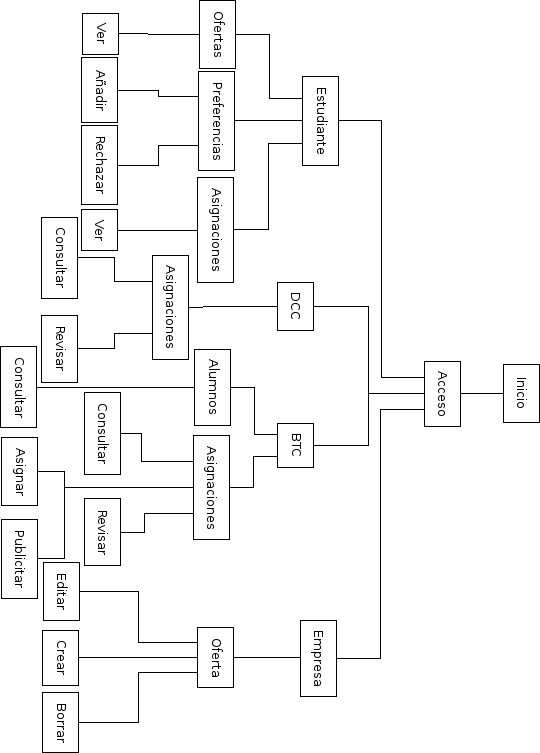
\includegraphics[width=\textwidth]{img/arbol_web}
\caption{\label{mapa_web} Mapa web con el acceso a los distintos contenidos.}
\end{center}
\end{figure}

\section{Diseño visual y definición de estilos}


A continuación se puede observar tres ejemplos de interfaces que hemos desarrollado para nuestra página web en las Figuras \ref{interfaz1}, \ref{interfaz2} y \ref{interfaz3}. Estas imagenes representan que es aquello que ve el usuario o el profesor con el rol BTC, viendo así como es el uso de la aplicación y el diseño empleado en la aplicación repetida durante todo el proceso.

\begin{figure}[h]
\begin{center}
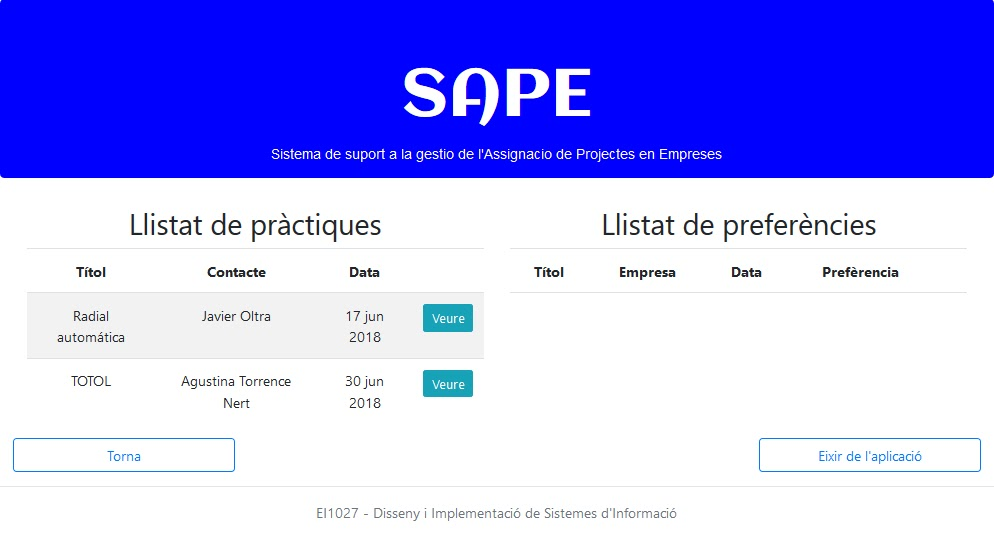
\includegraphics[width=\textwidth]{img/intefaz1.jpg}
\caption{\label{interfaz1}Esta interfaz permite al alumno puede ver y seleccionar sus preferencias de las prácticas que quiere realizar.}
\end{center}
\end{figure}

\begin{figure}[h]
\begin{center}
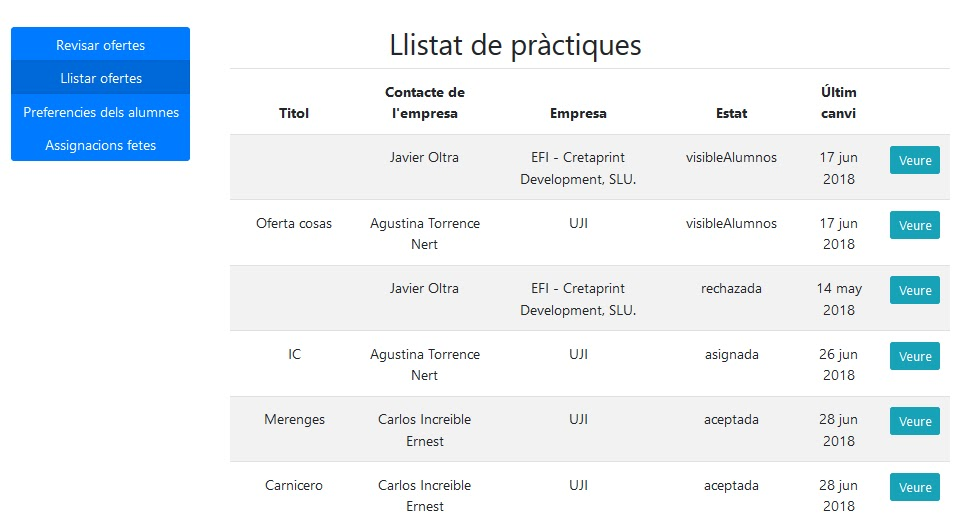
\includegraphics[width=\textwidth]{img/intefaz2.jpg}
\caption{\label{interfaz2}Esta interfaz permite al profesor con permisos BTC puede visualizar las prácticas y tener control sobre ellas.}
\end{center}
\end{figure}

\begin{figure}[h]
\begin{center}
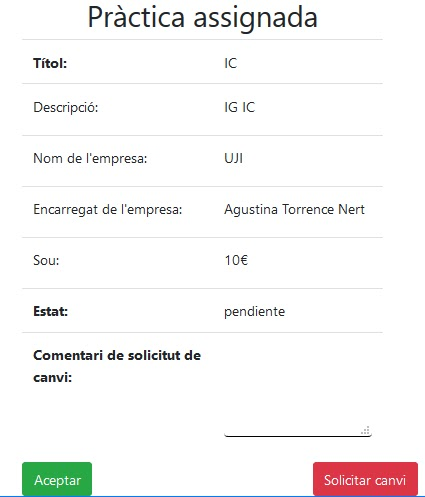
\includegraphics[width=\textwidth]{img/intefaz3.jpg}
\caption{\label{interfaz3}Esta interfaz permite al alumno aceptar o rechazar las prácticas de usuario asignadas por el profesor.}
\end{center}
\end{figure}

El propio equipo y también con la ayuda de familiares y amigos realizó distintos tipos de test enseñados a lo largo del curso, basándose principalmente en el material del profesorado \cite{evaluacion}.

Primero se expone el análisis heurístico realizado por el propio equipo. Las siguientes Figuras \ref{heuristico1}, \ref{heuristico2}, \ref{heuristico3}, \ref{heuristico4}, \ref{heuristico5}, \ref{heuristico6}, \ref{heuristico7}, \ref{heuristico8}, \ref{heuristico9}, \ref{heuristico10}, \ref{heuristico11}, \ref{heuristico12} y \ref{heuristico13} muestran los resultados obtenidos en el test, mostrando sólo el promedio recibido del total de las pruebas.

\begin{figure}[h]
\begin{center}
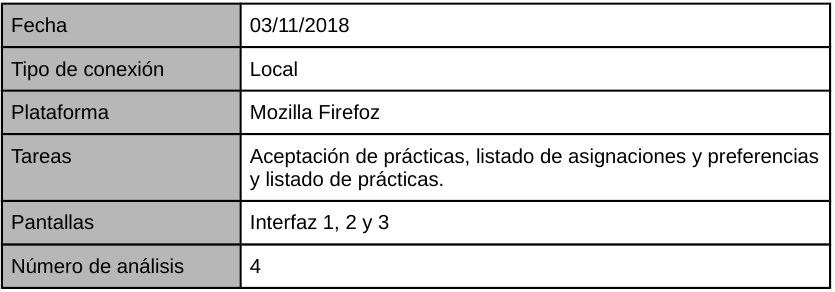
\includegraphics[width=\textwidth]{img/heuristico1}
\caption{\label{heuristico1}}
\end{center}
\end{figure}

\begin{figure}[h]
\begin{center}
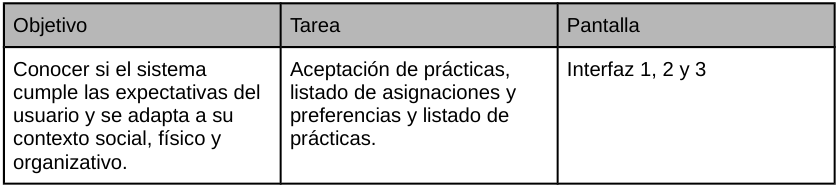
\includegraphics[width=\textwidth]{img/heuristico2}
\caption{\label{heuristico2}}
\end{center}
\end{figure}

\begin{figure}[h]
\begin{center}
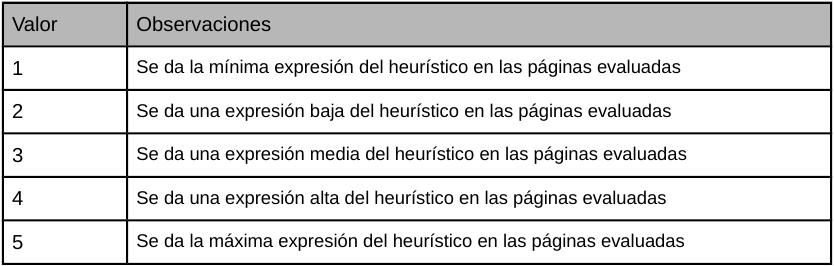
\includegraphics[width=\textwidth]{img/heuristico3}
\caption{\label{heuristico3}}
\end{center}
\end{figure}

\begin{figure}[h]
\begin{center}
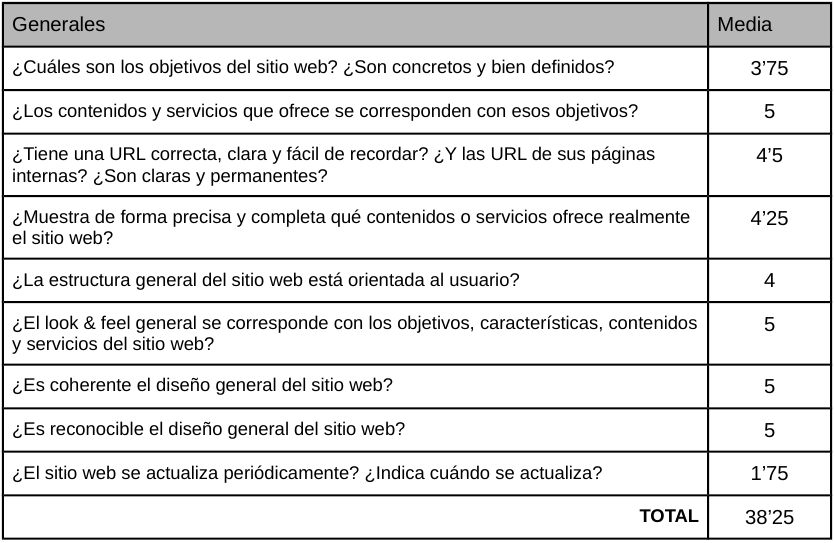
\includegraphics[width=\textwidth]{img/heuristico4}
\caption{\label{heuristico4}}
\end{center}
\end{figure}

\begin{figure}[h]
\begin{center}
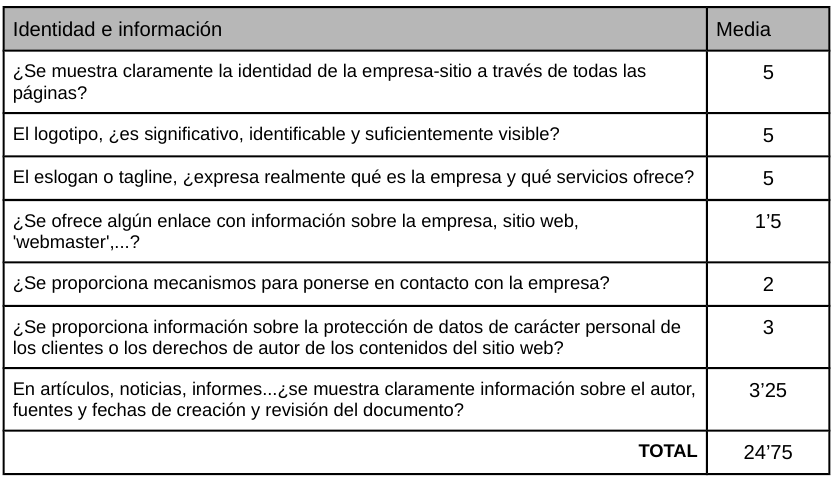
\includegraphics[width=\textwidth]{img/heuristico5}
\caption{\label{heuristico5}}
\end{center}
\end{figure}

\begin{figure}[h]
\begin{center}
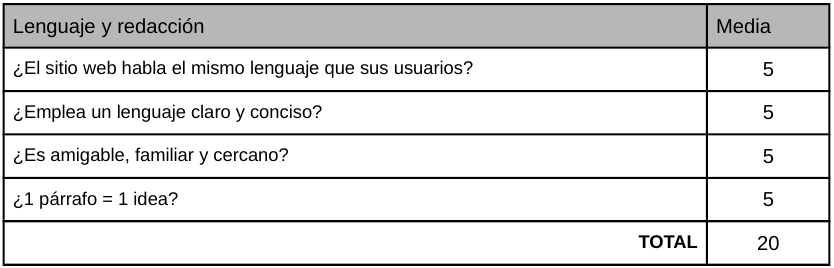
\includegraphics[width=\textwidth]{img/heuristico6}
\caption{\label{heuristico6}}
\end{center}
\end{figure}

\begin{figure}[h]
\begin{center}
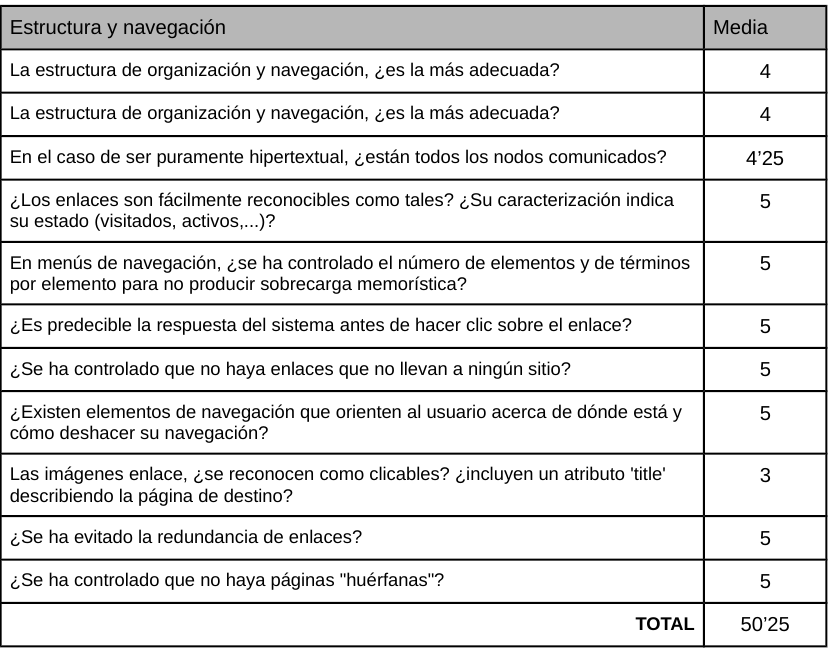
\includegraphics[width=\textwidth]{img/heuristico7}
\caption{\label{heuristico7}}
\end{center}
\end{figure}

\begin{figure}[h]
\begin{center}
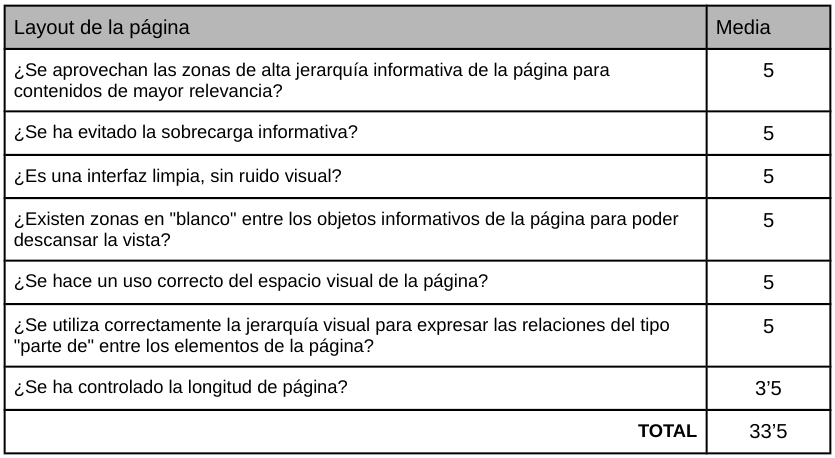
\includegraphics[width=\textwidth]{img/heuristico8}
\caption{\label{heuristico8}}
\end{center}
\end{figure}

\begin{figure}[h]
\begin{center}
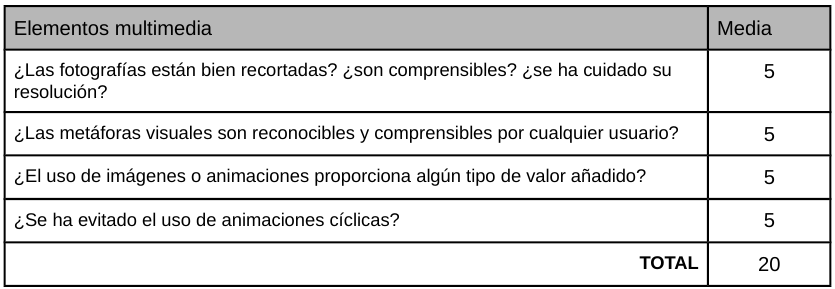
\includegraphics[width=\textwidth]{img/heuristico9}
\caption{\label{heuristico9}}
\end{center}
\end{figure}

\begin{figure}[h]
\begin{center}
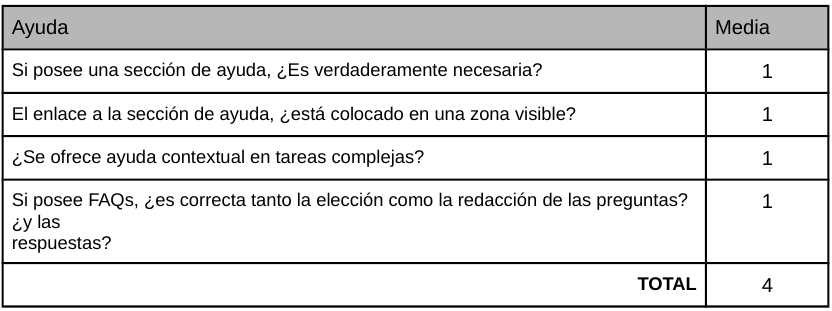
\includegraphics[width=\textwidth]{img/heuristico10}
\caption{\label{heuristico10}}
\end{center}
\end{figure}

\begin{figure}[h]
\begin{center}
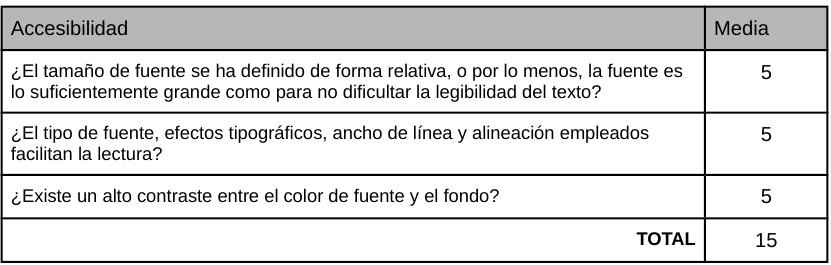
\includegraphics[width=\textwidth]{img/heuristico11}
\caption{\label{heuristico11}}
\end{center}
\end{figure}

\begin{figure}[h]
\begin{center}
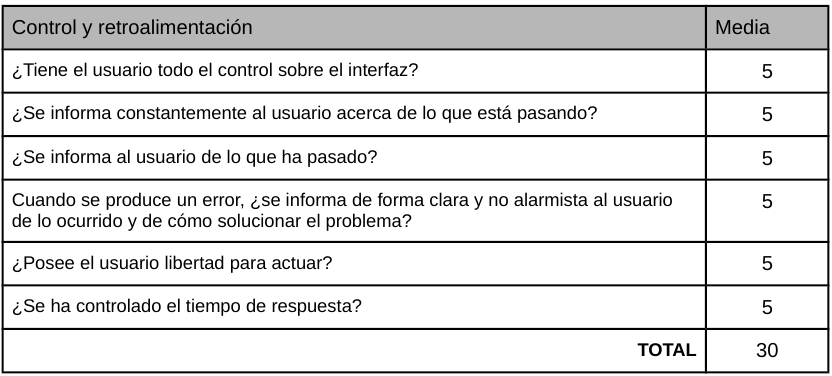
\includegraphics[width=\textwidth]{img/heuristico12}
\caption{\label{heuristico12}}
\end{center}
\end{figure}

\begin{figure}[h]
\begin{center}
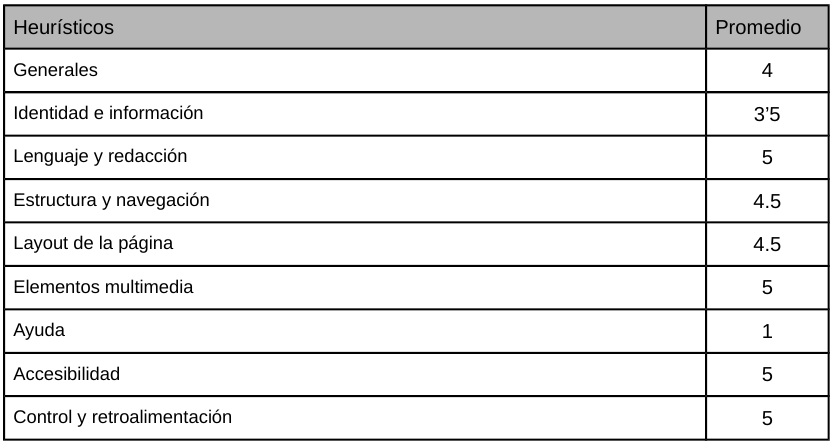
\includegraphics[width=\textwidth]{img/heuristico13}
\caption{\label{heuristico13}}
\end{center}
\end{figure}

Para una evaluación correcta de las interfaces también ha sido necesario la realización de un cuestionario de aceptación de usuarios. En la Figura \ref{test_usuarios} se puede observar el cuestionario realizado junto con el promedio sacado en las respuestas.

A partir de este resultado podemos observar que el resultado no resulta tan negativo, todo lo contrario. Ofrece una buena experiencia al usuario capaz de realizar las tareas de forma deseada.


\begin{figure}[h]
\begin{center}
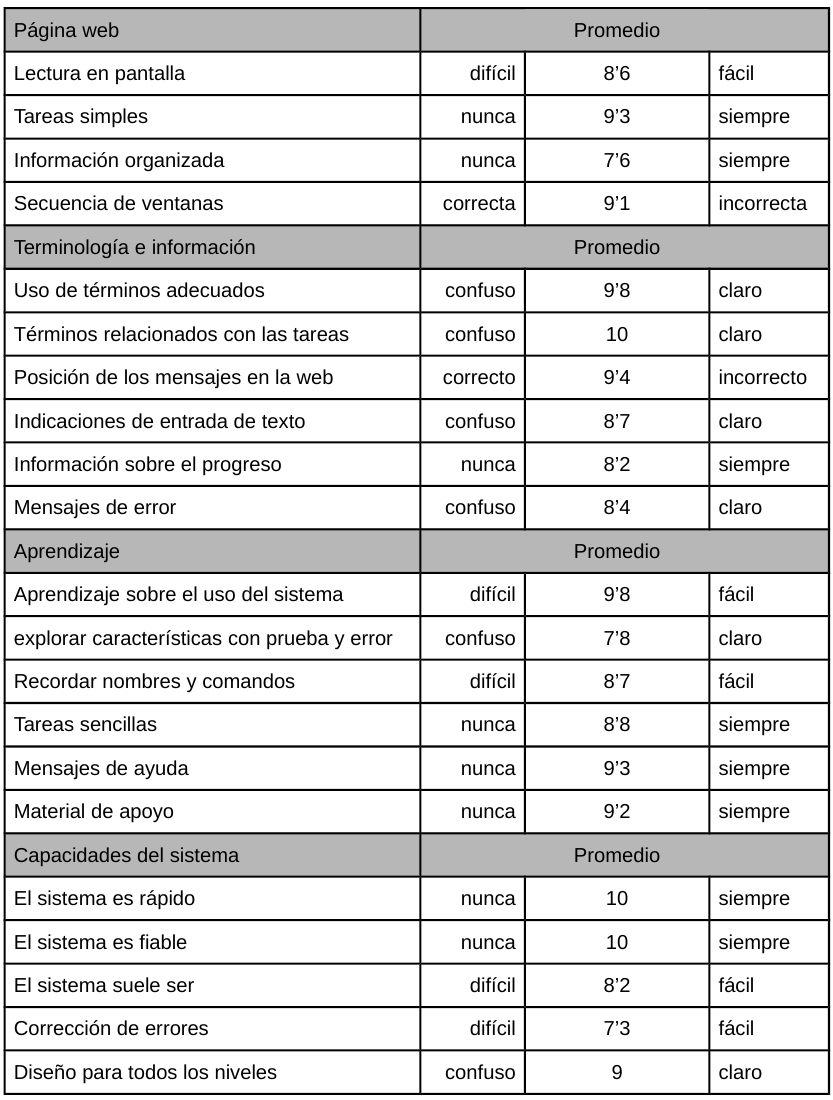
\includegraphics[width=\textwidth]{img/test_usuarios}
\caption{\label{test_usuarios}}
\end{center}
\end{figure}


\chapter{Implementación}

\section{Decisiones de implementación}

Durante el diseño de la página web realizada en la asignatura EI1027 - Diseño y implementación de sistemas de información, se ha realizado una estructura MVC (Modelo-Vista-Controlador) en el cual se han desarrollado todas las clases necesarias para el proyecto en las cuales se instancian todos los posibles usuarios de la pagina web.

También hay que mencionar que se han añadido diferentes roles en la base de datos, ya que dependiendo del rol que se tenga en la página se puede acceder a cierta información.

Por otra parte también se ha realizado varias páginas html, las cuales son las distintas páginas por las que los usuarios podrán navegar dependiendo de qué rol tienen. Por último se ha desarrollado una serie de controladores, los cuales, son los encargados de controlar el acceso a la base de datos.

\section{Control de errores}

Una vez se ha implementado el proyecto ha sido necesario un control de errores que valida los formularios de envío de información, ya que los usuarios no son perfectos y por lo tanto pueden tener errores a la hora de introducir datos en la página. 

Para ello se han implementado una serie de validadores para asegurarnos que los datos introducidos por el usuario son válidos y que, en caso de producirse un error durante su introducción, se informe de forma adecuada al usuario para que lo rectifique. Por último también ha sido necesario insertar ciertas restricciones para la correcta actualización de la base de datos. 

\section{Listado de paquetes y clases}

En este apartado encontramos las carpetas y ficheros en forma de árbol en la Figura \ref{arbol}, empleados en el desarrollo de la aplicación estando separados en las carpetas \emph{modelo}, \emph{dao} y \emph{controller} como bien se ha explicado en el apartado anterior por el \emph{MVC}.

\begin{itemize}
\item En el paquete \emph{controller} se encuentran almacenados los controladores de todas las clases y los validadores que se han implementado para la aplicación.
\item En el paquete \emph{dao} están las clases que acceden a nuestra base de datos.
\item En el paquete \emph{modelo} dispone de las clases que hemos utilizado en nuestro diagrama de clases para la implementación.
\end{itemize}

\verbatiminput{arbol.txt}
\begin{figure}[h]
\begin{center}
\caption{\label{arbol} Lista de ficheros empleados en el desarrollo de la aplicación empleando el patrón MVC.}
\end{center}
\end{figure}

\chapter{Conclusiones} 
Como conclusión hay que decir que el proyecto desarrollado en la asignatura EI1027 - Diseño e Implementación de Sistemas de información ha sido un proyecto que se ha desarrollado durado meses y que ha tenido una carga de trabajo bastante elevada.

Por otro lado es un proyecto muy completo en el que hemos visto todas las etapas para la realización de un sitio web de forma correcta, además de que ha sido un proyecto en el que hemos aprendido muchas herramientas, las cuales, seguro que utilizaremos en un futuro .

%Se pueden presentar conclusiones en varios aspectos: 
%en el ámbito formativo (sobre lo que has aprendido),
%en el ámbito profesional (sobre la experiencia en la empresa)
%y en el ámbito personal (sobre tu experiencia personal).
%En las conclusiones, además de las consideraciones personales, académicas o profesionales que el alumno quiera comentar, 
%se pueden incluir posibles extensiones del proyecto, así como la viabilidad comercial o empresarial cuando proceda.

Durante el desarrollo de la aplicación, se han adquirido nuevas competencias que se desconocían, como la resolución rápida de conflictos, la capacidad de documentar aplicaciones y las sinergias de trabajar en grupo.

Además la aplicación ha conseguido un funcionamiento bastante mejor del esperado, cumpliendo así los objetivos establecidos e incluidos a lo largo del curso.


% ------------------- Bibliografia ---------------------
\addcontentsline{toc}{chapter}{Bibliografía}
%\bibliographystyle{plane}
%\bibliography{MemoriaTecnicaBibliografia.bib}

\begin{thebibliography}{X}
\bibitem{caspractic}
 \textsc{María Cristina Campos Sancho},
 \textit{Cas per al treball de pràctiques de l'assignatura},
 \url{https://docs.google.com/document/d/16aIXg8UdvHcTzhVyMVpaHZVP_KefRawoehEIr81dRNc/},
  29 de octubre de 2018.
\bibitem{presentacion}
 \textsc{Ismael Sanz},
 \textit{Introducció a la usabilitat i el disseny d'interfícies},
 \url{https://docs.google.com/presentation/d/18kpzN31lZoxK2hXcdZPjD_FLBBdm8KG5-db__kYjlKk/},
  29 de octubre de 2018.
\bibitem{ejercicio}
 \textsc{Lledó Museros Cabedo},
 \textit{Exercici Disseny d’interfícies d’usuari centrat en l’usuari},
 \url{https://docs.google.com/document/d/1g6bx4PCpFXTPRI6hy8UcK9XvFo6obJrpJBEnpC1UlSk/},
  29 de octubre de 2018.
\bibitem{evaluacion}
 \textsc{Lledó Museros Cabedo e Ismael Sanz},
 \textit{Avaluació de llocs web},
 \url{https://docs.google.com/presentation/d/1wMODQ3NZlBf_bLPlPbN0X8dh-wjywwT8cy9EgVYpTh4/},
  29 de octubre de 2018.
\end{thebibliography}


% ------------------- Anexos ---------------------

\appendix
%\renewcommand\appendixname{Anexo}

% ---- Primer Anexo ----
%\chapter{Estudio detallado de...}

%\section{Definición}

%\section{Aplicaciones}

% ---- Segundo Anexo ----
%\chapter{Tablas de ...}

\end{document}
